\subsection{sPHENIX Collected Datasets}
Runs during the physics quality RHIC Run 2024 \pp collision period were used for this analysis. 
These runs were selected based on high calorimeter and global detector data quality similar to the selection criteria used in the previous analysis (Section~\ref{sec:detdeta_datasets}).
Data was collected using a hardware level calorimeter patch ``Jet'' trigger.
This ``Jet'' trigger used a jet-patch algorithm to search $\Delta\eta \times \Delta\phi = 0.8 \times 0.8$ overlapping windows for the highest total energy from all towers in the three calorimeter layers (EMCal, IHCal, and OHCal) in that region. 
The jet trigger used in this analysis corresponds to approximately energy thresholds within the patch of 10~\GeV.
A set of offline event selection criteria was also applied to the data to select a clean set of inclusive and dijet events for this analysis.
More details on the offline event selection used to select jet events for this analysis is outlined in Section~\ref{sec:ueinpp_selection}.

\subsection{Monte Carlo Datasets}
\label{sec:mc_samples}
Two MC generators, \pythia and \herwig, are used for comparison to data and for deriving response matrix information when unfolding detector-level results of the underlying event back to the truth level.
A total of eleven samples, filtered across a range of jet trigger thresholds, are used to cover the phase space of \pp jet events at \snn = 200 GeV.
For both the \pythia and \herwig generators, each sample is generated with a minimum hard-scattering \pT{} threshold to ensure sufficient statistical precision in the high-\pT{} jet region.
Events are subsequently filtered using R=0.4 anti-$k_T$ jets formed from generator-level stable particles to ensure the events have a generator-level leading jet above the desired \pT{} threshold for that jet sample within the detector acceptance.
The quoted cross sections for each sample include the efficiency correction of this filtering step and are used to weight the samples when combining them.
The final combined distributions are obtained using weights based on the filtered cross section and the number of events in each dataset.
Finally, the fully efficient truth-level leading jet \pT{} ranges for each sample are determined by matching the resulting spectra to those from minimum-bias and/or lower-threshold filtered samples, ensuring a consistent description across overlapping regions of phase space. 
These events were then passed through the full sPHENIX detector \geant~\cite{GEANT4} simulation and reconstruction to produce simulation datasets that can be compared directly to data.
The MC events are also reweighted to match the z-vertex distribution and calorimeter pedestal noise level in data during the 2024 p+p running. 
The full set of MC sample details used in the analysis are included in Table~\ref{table:MCdataset}.

\begin{table}[ht]    
\centering
\begin{tabular}{|c|cccc|}
\hline
Lead Jet $p_T$ range [GeV] & Min $\hat{p_{T}}$ [GeV] & Generator & $\sigma$ [pb] & $N_{events}$ \\ \hline
14-21 & MB & Pythia8   & 1.4903e+06 & 10M   \\ \hline
21-32 & 10 & Pythia8   & 6.2623e+04 & 10M   \\ \hline
32-42 & 15 & Pythia8   & 2.5298e+03 & 10M   \\ \hline
42-52 & 22 & Pythia8   & 1.3553e+02 & 10M   \\ \hline
52-62 & 29 & Pythia8   & 7.3113     & 10M   \\ \hline
62+   & 36 & Pythia8   & 3.3261e-01 & 10M   \\ \hline
14-21 & MB & Herwig    & 6.7108e+05 & 10M   \\ \hline
21-32 & 10 & Herwig    & 5.2613e+04 & 10M   \\ \hline
32-42 & 15 & Herwig    & 2.0694e+03 & 10M   \\ \hline
42-52 & 22 & Herwig    & 1.0510e+02 & 10M   \\ \hline
52+   & 29 & Herwig    & 5.2089     & 10M   \\ \hline
\end{tabular}
\caption{Summary of MC samples with generator, cross section and number of events information.}
\label{table:MCdataset} 
\end{table}

\subsubsection{Monte Carlo Sample Combination}
As a validation step on the cross section weights determined from the \pythia cross section values and filtering weights for each triggered MC sample, the truth and reconstructed leading jet spectra are shown in Figure~\ref{fig:mc_sample_distributions}. 
A smooth transition between jet $p_{T}$ range samples is seen for both the truth leading jet $p_{T}$ distribution and the reconstruction-level leading jet $p_{T}$ distribution. 
Note, as further described in the event selection criteria outlined in Section~\ref{sec:ueinpp_selection}, jet $p_{T}$ threshold cuts are applied in the analysis of 17 GeV in truth leading jet $p_{T}$ and 21 GeV in reconstructed leading jet $p_{T}$. However, Figure~\ref{fig:mc_sample_distributions} includes contributions from below these thresholds to account for resolution effects smearing the jet $p_{T}$ distribution. 

Figure~\ref{fig:mc_sample_distributions} also shows the contributions to the transverse region $E_{T}$ measurement from each of the triggered MC samples.
It is this variable, the average total transverse region $E_{T}$, that is actually used in the analysis calculate the underlying event measurement. 
The truth transverse region $E_{T}$ distribution is determined by summing the $E_{T}$ of all final state particles in the transverse region, while the reconstructed transverse region $E_{T}$ distribution is determined by summing the $E_{T}$ of all calorimeter topoclusters in the transverse region.
In these plots, there is strong overlap in the $E_{T}$ spectra for different jet triggered samples as well as the extent to which the $E_{T}$ distribution extends out which helps to determine what a reasonable high $E_{T}$ threshold is for the $E_{T}$ axes of the unfolding response matrix and measured histograms.
Therefore, for the truth $\Sigma E_{T}$ distribution, a maximum $\Sigma E_{T}$ of 35 GeV is considered in the analysis, while for the reconstructed $\Sigma E_{T}$ distribution, a maximum $\Sigma E_{T}$ of 20 GeV is considered.
Additional information on the topocluster reconstruction and UE measurement calculation is included in Section~\ref{sec:ueinpp_towerreco}.

\begin{figure}
    \centering
    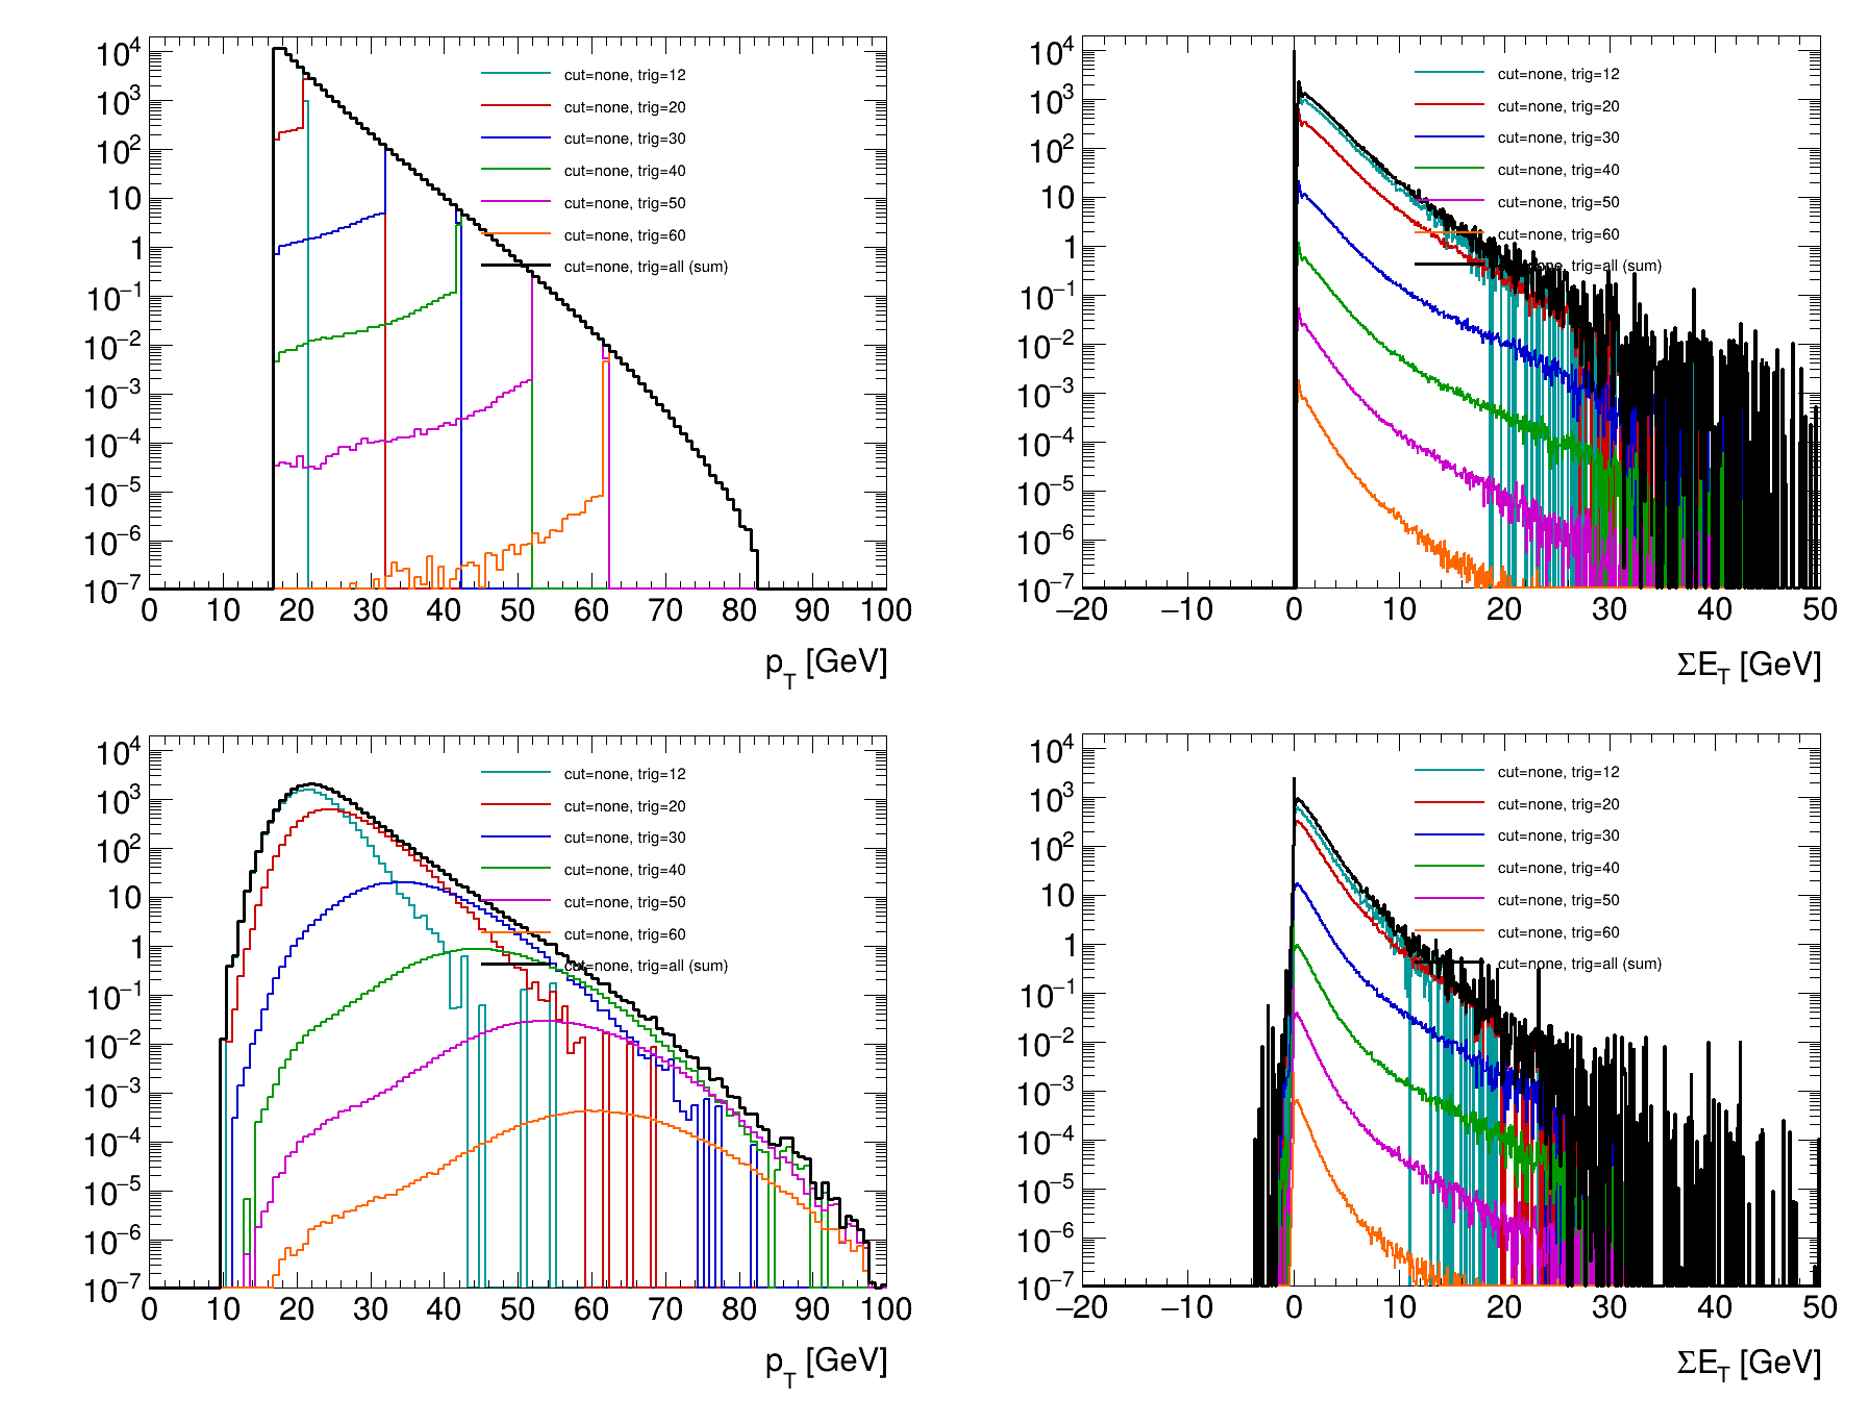
\includegraphics[width=\linewidth]{ueinpp/Figures/unfolding/MC_sample_distributions_inclusive.png}
    \caption{Plots of truth leading jet $p_{T}$ spectra (top left), reconstruction level calibrated leading jet $p_{T}$ spectra (top right), truth transverse region $E_{T}$ (bottom left) and reconstruction level transverse region $E_{T}$ (bottom right) for each MC triggered sample and the full MC distribution with cross section weighting.}
    \label{fig:mc_sample_distributions}
\end{figure}

\subsubsection{Monte Carlo Vertex Reweighting}
\label{sec:mc_vertex_reweighting}

Monte Carlo events are also reweighted to match the $z_{\mathrm{vtx}}$ distribution observed in data. 
The same procedure used for the $z_{\mathrm{vtx}}$ reweighting in the previous analysis (Section~\ref{sec:detdeta_datasets}) is applied here, where a weight is calculated for each MC event based on the $z_{\mathrm{vtx}}$ distribution in data and the $z_{\mathrm{vtx}}$ distribution in MC.

The effect of this reweighting is evaluated at both truth and reconstructed levels. 
Figure~\ref{fig:vertex_reweighting} compares truth leading jet $p_{T}$, truth transverse region $\Sigma E_{T}$, calibrated leading jet $p_{T}$, and reconstruction-level transverse region $\Sigma E_{T}$ distributions before and after vertex reweighting.
No significant modification for the truth or reconstructed jet and $E_{T}$ distributions is observed. 

\begin{figure}
    \centering
    \begin{subfigure}[t]{0.48\linewidth}
        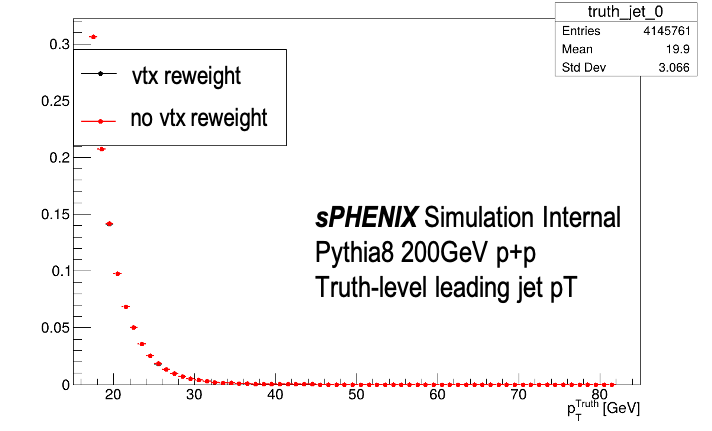
\includegraphics[width=\linewidth]{ueinpp/Figures/unfolding/mc_vertex_reweight_truthjet.png}
        \caption{Truth leading jet $p_{T}$}
    \end{subfigure}
    \hfill
    \begin{subfigure}[t]{0.48\linewidth}
        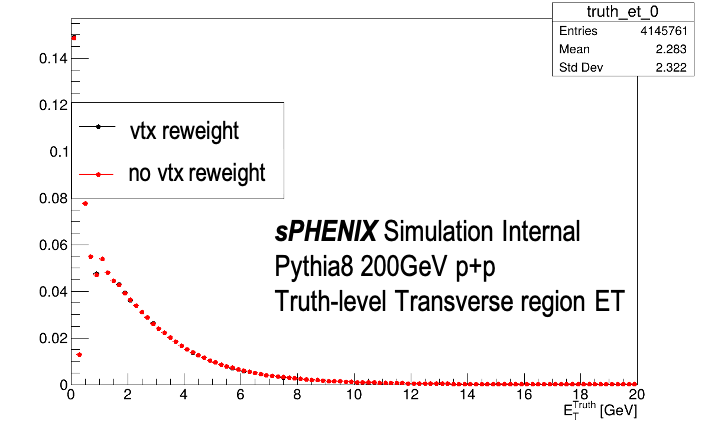
\includegraphics[width=\linewidth]{ueinpp/Figures/unfolding/mc_vertex_reweight_truthet.png}
        \caption{Truth transverse region $\Sigma E_{T}$}
    \end{subfigure}
    \vspace{0.4em}
    \begin{subfigure}[t]{0.48\linewidth}
        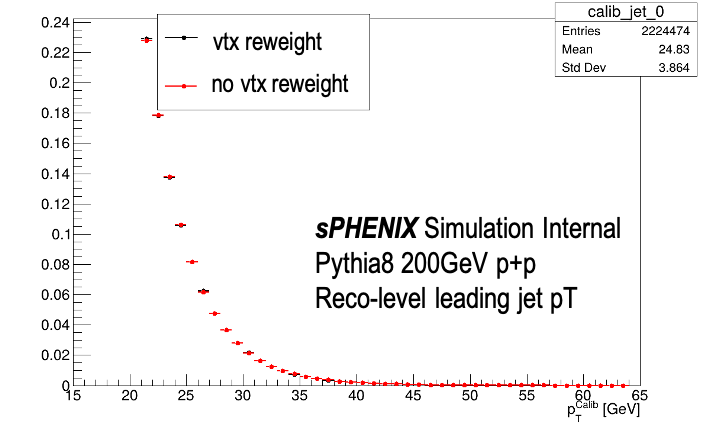
\includegraphics[width=\linewidth]{ueinpp/Figures/unfolding/mc_vertex_reweight_calibjet.png}
        \caption{Reconstructed leading jet $p_{T}$}
    \end{subfigure}
    \hfill
    \begin{subfigure}[t]{0.48\linewidth}
        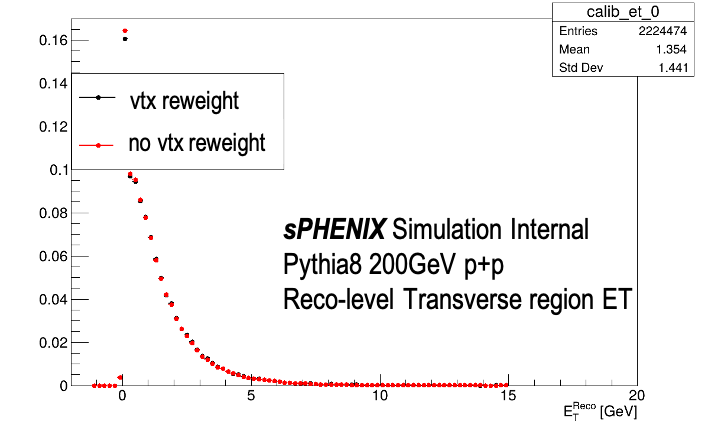
\includegraphics[width=\linewidth]{ueinpp/Figures/unfolding/mc_vertex_reweight_recoet.png}
        \caption{Reconstructed transverse region $\Sigma E_{T}$}
    \end{subfigure}
    \caption{Distributions of leading jet $p_{T}$ and transverse region $\Sigma E_{T}$ before and after MC vertex reweighting at truth and reconstruction levels.}
    \label{fig:vertex_reweighting}
\end{figure}